\documentclass[a4page,notitlepage]{article}
\usepackage{color,amsmath,graphicx,subcaption,geometry,mathtools}
\usepackage{cite}
\usepackage{mhchem}
\usepackage[dvipsnames]{xcolor}
\usepackage{tikz}
\usepackage{pgfplots}
\usepackage{stackengine,ifthen}
\usetikzlibrary{arrows,positioning,calc}
\newcommand\influx{0.5}

\newenvironment{customlegend}[1][]{
  \begingroup
  \csname pgfplots@init@cleared@structures\endcsname
  \pgfplotsset{#1}
}{
  \csname pgfplots@createlegend\endcsname
  \endgroup
}

\def\addlegendimage{\csname pgfplots@addlegendimage\endcsname}
\setlength\abovecaptionskip{6pt}
\providecommand{\abs}[1]{\lvert#1\rvert}
\providecommand{\norm}[1]{\lVert#1\rVert}


\title{Kinetic parameters of enzymes are constrained by stable functioning of autocatalytic cycles}
\author{Uri Barenholz, Dan Davidi, Yinon Bar-On, Elad Noor, Niv Antonovsky, Ron Milo, \dots}
\date{}

\begin{document}
\maketitle
\abstract{
    Autocatalytic cycles are an important part of metabolic networks.
    As the flux in autocatalytic cycles both depends on the concentration of intermediate metabolites and affects it, they present unique features and characteristics.
    We use an automated process to identify autocatalytic cycles in central carbon metabolism.
    We show that even very simple cycles impose specific constraints on the kinetic parameters of the enzymes composing them and their expression levels, in order to allow stable, non-zero fluxes.
    We find these constraints to hold for functioning autocatalytic cycles for which data is available.

    We analyze a simple, generic metabolic autocatalytic cycle, presenting the mathematical tools and techniques needed in order to gain insights about its operation.
    We derive the relationships between two global traits of the cycle: (A) having a non-zero flux steady state, and (B) requiring that the non-zero steady state is stable, and the kinetic parameters of the enzymes forming the cycle.
    We show that the autocatalytic reaction must have higher affinity and lower maximal flux than the reaction diverting metabolites out of the cycle for biomass generation, for stable fluxes through the cycle to occur.
    We discuss various extensions of the simple model including different kinetic functions and external fluxes into the cycle.
    We give examples of autocatalytic cycles occurring in central carbon metabolism, which are generally not considered as such, and for which our conclusions can be applied.
    We find our analysis to be valid on cases for which sufficient data is available.
    This work thus serves as an approachable introduction to the analysis of autocatalytic metabolic cycles and as a demonstration of the insights one can get by such analysis on real networks.
}

\section{Introduction}
    Autocatalysis is generally defined as a setup in which one of the products of a chemical reaction is also a reactant in the same, or coupled reaction (see, for example, \cite{Steinfeld1999-iw}).
    A metabolic cycle is a set of reactions and metabolites such that the reactions form a cycle with respect to the metabolites, allowing metabolites external to the cycle to serve as additional reactants or products of the reactions.
    A metabolic cycle is autocatalytic if traversing the reactions that form the cycle increases the amount of the metabolites forming it.
    Surprisingly, autocatalytic cycles can be an essential building block of optimal metabolic networks \cite{Riehl2010-yh}.

    Autocatalytic cycles present specific metabolic control challenges as their inherent feed-back nature makes them susceptible to divergence or drainage \cite{Fell1999,Reznik2010-te}.
    An understanding of the unique constraints that metabolic autocatalytic cycles impose is therefore essential for realizing limitations of existing metabolic networks, as well as for the introduction of modifications to them in synthetic biology metabolic engineering applications.

    The importance of autocatalytic cycles in metabolism is demonstrated by one of its most prominent examples, the Calvin Benson Bassham cycle (CBB) \cite{Benson1950-cl}.
    The CBB cycle, assimilating \ce{CO2} to convert 5-carbon compounds to 6-carbon compounds, serves as the main gateway for converting inorganic carbon to organic compounds in nature \cite{Raven2012-le}.
    As we observe below, more autocatalytic cycles exist in central carbon metabolism suggesting important biological insights can be gained by understanding the constraints underlying their stable operation.

    In this work we present the specific requirements autocatalytic cycles must meet in order to operate: (A) To be able to achieve at least one, non-zero, steady state of fluxes; 
    (B) To be stable for fluctuations at the steady state point(s).
    The mathematical tools we define and use are widely known and applicable in various fields (see, for example \cite{Strogatz2014-hp}).
    Our analysis demonstrates the use of these tools to gain insights about the operation, limitations, and various modifications available to metabolic autocatalytic cycles in vivo.

\section{Autocatalytic cycles play important roles in central carbon metabolism}

While a few autocatalytic cycles are widely known, the definition we use for autocatalysis yields several autocatalytic cycles in central carbon metabolism that are not usually considered as such.
In this work, we define an autocatalytic cycle as a set of reactions and metabolites that satisfy the following conditions:
(A) Cyclicity w.r.t. the metabolites, namely that each metabolite serves both as a substrate of at least one reaction of the cycle and as a product of at least one reaction of the cycle.
(B) Cyclicity w.r.t. the reactions, namely that at least one substrate of each reaction, and one product of each reaction are metabolites of the cycle.
(C) Autocatalysis, namely that there is a set of positive integers corresponding to the reactions forming the cycle, such that the result of applying all of the reactions in the cycle, each at its corresponding integer number of times, will overall increase the amount of at least one metabolite in the cycle, and will not decrease the amount of any of the other metabolites in the cycle.

We implemented an algorithm to search for autocatalytic cycles in central carbon metabolism.
The algorithm identified 4 classes of autocatalytic cycles, where for some classes a few different variations were identified.
We note that our algorithm is incomplete, meaning additional autocatalytic cycles may exist in central carbon metabolism.
Moreover, our algorithm is not optimized, resulting in an exponential increase in identified cycles when executed on the full metabolic network of \emph{E.coli} due to combinatorial combinations of elementary cycles to composite ones.
Further work will enable a more robust algorithm to identify more autocatalytic cycles in the metabolic network.

Representatives of the different classes of cycles identified  are presented in figure \ref{fig:realautocatal}.
These classes are:
(A) The glyoxylate cycle that can be used to produce two malate molecules from a single isocitrate molecule, assimilating acetyl-CoA, then converting the two malate molecules back into two isocitrate molecules \cite{Kornberg1966-lh};
(B) Cycles using phosphoenolpyruvate (PEP) to transport substrates using the phosphotransferase system (PTS), then converting the imported substrate into two PEP molecules;
(C) Various parts of the pentose phosphate cycle assimilating either erythrose-4P, sedoheptulose-7P, or both, to produce 5, 3 and 6 carbon compounds at higher stoichiometries;
(D) Cycles assimilating glycerone phosphate using the fructose bisphosphate aldolase reaction in the reverse direction, producing fructose 1,6 bisphosphate from glyceraldehyde 3 phosphate, then converting the fructose back into two glyceraldehyde 3 phosphate using the Entner Doudoroff (ED) pathway \cite{Entner1952-xs}.

The amount of autocatalytic cycles we identified suggests that the unique features of autocatalytic cycles may confine and shape the kinetic parameters of a broad set of enzymes central to metabolism.

\begin{figure}[h!]
\centering
\includegraphics[scale=0.86]{central-carbon-met-fig1.pdf}
    \caption {
    Examples of 5 autocatalytic cycles in central carbon metabolism.
    The reactions forming each cycle are highlighted in blue.
    The metabolite colored in magenta is the metabolite more molecules of which are produced when the cycle is traversed.
    The metabolite colored in teal is the metabolite assimilated by the cycle.
    Upper panel represents the cycles on top of the central carbon metabolism network.
    Lower panel represents the isolated cycles, with dashed blue arrows indicating the omission of intermediate metabolites and reactions.
(A) The glyoxylate cycle, producing two malate molecules from a single isocitrate molecule, assimilating acetyl-CoA;
(B) A cycle using PEP to transport glucose using the PTS, then converting the imported glucose into two PEP molecules;
(C) A representative of a class of autocatalytic cycles using parts of the pentose phosphate cycle, the presented variant assimilates sedoheptulose-7P to produce fructose 6 phosphate from glyceraldehyde 3 phosphate;
(D) A cycle assimilating glycerone phosphate using the fructose bisphosphate aldolase reaction in the reverse direction, producing fructose 1,6 bisphosphate from glyceraldehyde 3 phosphate, then converting the fructose back into two glyceraldehyde 3 phosphate;
(E) The Calvin Benson Bassham cycle assimilating \ce{CO2} to convert ribulose bis phosphate to two glycerate 3 phosphate, then recycling the 3 carbon substrate through the pentose phosphate cycle back to ribulose.}
    \label{fig:realautocatal}
\end{figure}

\section{Analysis of a simple autocatalytic cycle}
    We consider the simple autocatalytic cycle depicted in Figure \ref{fig:simplecycle}A.
    This cycle has a single intermediate metabolite, $X$, one autocatalytic reaction with flux $f_a$, such that for any unit of $X$ consumed, it produces two units of $X$ (this reaction obviously consumes some external metabolite, which we assume to be at a constant concentration), and one outgoing reaction using the cycle substrate with flux $f_b$.
    We assume simple, irreversible Michaelis-Menten kinetics for the two reactions such that:
    \begin{eqnarray*}
      f_a = \frac{V_{\max,a}X}{K_{M,a}+X} \\
      f_b = \frac{V_{\max,b}X}{K_{M,b}+X}
    \end{eqnarray*}
    where all the kinetic parameters are positive.
    \begin{figure}[h!]
      \begin{minipage}[c]{.3\linewidth}%
        {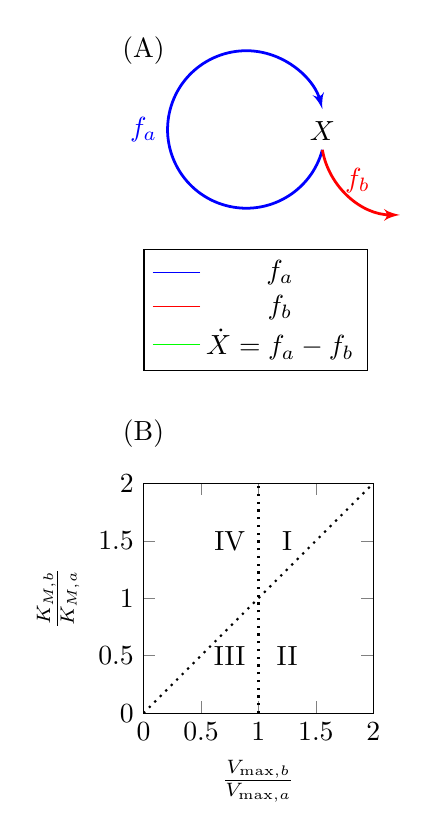
\begin{tikzpicture}[>=latex',node distance = 2cm]
            \node (X) {$X$};
            \draw [->,line width=1pt,blue] (X.south) arc (345:15:1cm) node [pos=0.5,left] (fa) {$f_a$};
            \draw [->,line width=1pt,red] (X.south) arc (190:270:1cm) node [pos=0.3,right] {$f_b$};
            \node [above of=fa,yshift=-1cm] (A) {(A)};
            \begin{customlegend}[legend entries={$f_a$,$f_b$,$\dot{X}=f_a-f_b$},legend style={below=2cm of fa,anchor=west,name=legend1}]
              \addlegendimage{blue,fill=black!50!red,sharp plot}
              \addlegendimage{red,fill=black!50!red,sharp plot}
              \addlegendimage{green,fill=black!50!red,sharp plot}
            \end{customlegend}
            \begin{axis}[name=phase,xmin=0,ymin=0,xmax=2,ymax=2,xlabel={$\frac{V_{\max,b}}{V_{\max,a}}$},ylabel={$\frac{K_{M,b}}{K_{M,a}}$},samples=6,at=(legend1.south west),anchor=above north west,width=4.5cm,height=4.5cm,yshift=-1.2cm]
            \addplot[domain=0:4,dotted,black,thick] {x};
            \addplot[dotted,black,thick] coordinates {(1,0) (1,2)};
            \node (one) at (axis cs:1.25,1.5) {I};
            \node (two) at (axis cs:1.25,0.5) {II};
            \node (three) at (axis cs:0.75,0.5) {III};
            \node (four) at (axis cs:0.75,1.5)(axis cs:1.25,0.5) {IV};
          \end{axis}
          \node [at=(legend1.south west),yshift=-0.8cm] (B) {(B)};
         \end{tikzpicture}}%
       \end{minipage}
       \hfill
       \begin{minipage}[c]{.65\linewidth}
        {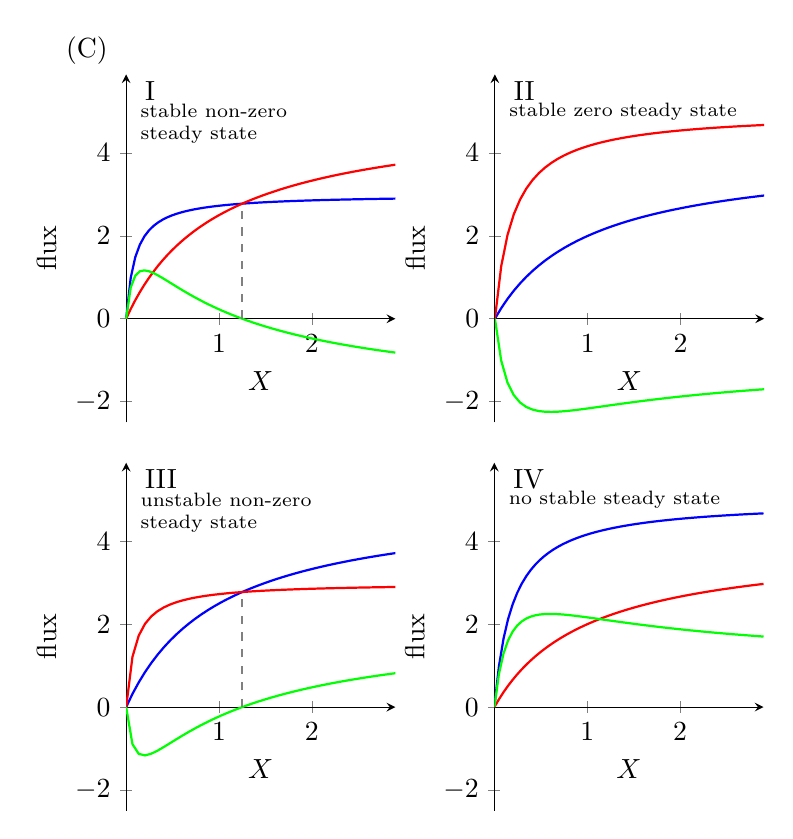
\begin{tikzpicture}
            \begin{axis}[name=plot1,axis x line=middle,axis y line=left,xlabel near ticks,ylabel near ticks,xmin=0,ymin=-2.5,xmax=2.9,ymax=5.9,xlabel={$X$},ylabel={flux},samples=60,width=5cm,height=6cm,clip=false]
            \addplot[domain=0:2.9,blue,thick] {3*x/(0.1+x)};
            \addplot[domain=0:2.9,red,thick] {5*x/(1+x)};
            \addplot[domain=0:2.9,green,thick] {3*x/(0.1+x)-5*x/(1+x)};
            \addplot[dashed,gray,thick] coordinates {(1.25,0) (1.25,2.77)};
            \node[right] (one) at (axis cs:0.1,5.5) {I};
            \node[right,align=left] (onetext) at (axis cs:0.05,4.7) {\scriptsize stable non-zero\\[-0.4em]\scriptsize steady state};
          \end{axis}
          \node [at=(plot1.north west),xshift=-0.5cm,yshift=0.3cm] (C) {(C)};

          \begin{axis}[name=plot2,axis x line=middle,axis y line=left,xlabel near ticks,ylabel near ticks,xmin=0,ymin=-2.5,xmax=2.9,ymax=5.9,xlabel={$X$},ylabel={flux},samples=60,at=(plot1.right of south east),anchor=left of south west,width=5cm,height=6cm]
            \addplot[domain=0:4,blue,thick] {4*x/(1+x)};
            \addplot[domain=0:4,red,thick] {5*x/(0.2+x)};
            \addplot[domain=0:4,green,thick] {4*x/(1+x)-5*x/(0.2+x)};
            \node[right] (two) at (axis cs:0.1,5.5) {II};
            \node[right,align=left] (twotext) at (axis cs:0.05,5) {\scriptsize stable zero steady state};
          \end{axis}

          \begin{axis}[name=plot3,axis x line=middle,axis y line=left,xlabel near ticks,ylabel near ticks,xmin=0,ymin=-2.5,xmax=2.9,ymax=5.9,xlabel={$X$},ylabel={flux},samples=60,at=(plot1.below south west),anchor=above north west,width=5cm,height=6cm,yshift=-0.5cm]
            \addplot[domain=0:4,blue,thick] {5*x/(1+x)};
            \addplot[domain=0:4,red,thick] {3*x/(0.1+x)};
            \addplot[domain=0:4,green,thick] {5*x/(1+x)-3*x/(0.1+x)};
            \addplot[dashed,gray,thick] coordinates {(1.25,0) (1.25,2.77)};
            \node[right] (three) at (axis cs:0.1,5.5) {III};
            \node[right,align=left] (threetext) at (axis cs:0.05,4.7) {\scriptsize unstable non-zero\\[-0.4em]\scriptsize steady state};
          \end{axis}

          \begin{axis}[name=plot4,axis x line=middle,axis y line=left,xlabel near ticks,ylabel near ticks,xmin=0,ymin=-2.5,xmax=2.9,ymax=5.9,xlabel={$X$},ylabel={flux},samples=60,at=(plot3.right of south east),anchor=left of south west,width=5cm,height=6cm]
            \addplot[domain=0:2.9,blue,thick] {5*x/(0.2+x)};
            \addplot[domain=0:2.9,red,thick] {4*x/(1+x)};
            \addplot[domain=0:2.9,green,thick] {5*x/(0.2+x)-4*x/(1+x)};
            \node[right] (four) at (axis cs:0.1,5.5) {IV};
            \node[right,align=left] (fourtext) at (axis cs:0.05,5) {\scriptsize  no stable steady state};
         \end{axis}
        \end{tikzpicture}}
       \end{minipage}
      \caption{\label{fig:simplecycle}
        (A) A simple autocatalytic cycle induces two fluxes, $f_a$ and $f_b$ as a function of the concentration of $X$.
        These fluxes follow simple Michaelis Menten kinetics.
        A steady state occurs when $f_a=f_b$, implying that $\dot{X}=0$.
        The cycle always has a steady state at $X=0$.
        The slope of each reaction at $X=0$ is $V_{\max}/K_m$.
        A steady state is stable if at the steady state point $\frac{d\dot{X}}{dX}<0$.
        (B) Each set of kinetic parameters, $V_{\max,a},V_{\max,b},K_{M,a},K_{M,b}$ results in one of four cases (C): 
       (I) there is a stable positive steady state and zero is an unstable steady state; 
       (II) zero is the only non-negative steady state, and it is stable;
       (III) zero is a stable steady state and there is a positive, non-stable steady state; 
       (IV) zero is the only non-negative steady state and it is unstable.}
    \end{figure}

    We characterize the metabolic state of this system by the concentration of the metabolite $X$.
    We note that knowing the concentration of $X$ suffices in order to calculate the fluxes originating from it, $f_a$ and $f_b$, thus fully defining the state of the system.
    A steady state of the system is defined as a concentration, $X^*$, which induces fluxes that keep the concentration steady, such that the total in-flux to $X$ is exactly equal to the total out-flux from it.
    In our example, the outgoing flux from $X$ is $f_a+f_b$ and the incoming flux to $X$ is $2f_a$, so at steady state it holds that:
    \begin{equation}
      \label{eq:xdyna}
      \dot X = \frac{dX}{dt} = 2f_a - (f_a + f_b) = 0
    \end{equation}

    Expanding this condition we get:
    \begin{equation*}
      \dot X = 0 \Rightarrow f_a = f_b \Rightarrow \frac{V_{\max,a}X}{K_{M,a}+X}=\frac{V_{\max,b}X}{K_{M,b}+X}
    \end{equation*}
    which is satisfied either if $X=0$ or if:
    \begin{equation}
      \label{eq:xstst}
      X=\frac{V_{\max,b}K_{M,a}-V_{\max,a}K_{M,b}}{V_{\max,a}-V_{\max,b}}
    \end{equation}
    As physiologically the concentration of $X$ cannot be negative, we get a constraint on the kinetic parameters for which a positive steady state exists:
    \begin{equation*}
      \frac{V_{\max,b}K_{M,a}-V_{\max,a}K_{M,b}}{V_{\max,a}-V_{\max,b}}>0 \Rightarrow \frac{\frac{V_{\max,b}}{K_{M,b}}-\frac{V_{\max,a}}{K_{M,a}}}{V_{\max,a}-V_{\max,b}}>0
    \end{equation*}
    The constraint states that if $V_{\max,a}>V_{\max,b}$ then it must be that $\frac{V_{\max,b}}{K_{M,b}}>\frac{V_{\max,a}}{K_{M,a}}$ and that if $V_{\max,a}<V_{\max,b}$ then $\frac{V_{\max,b}}{K_{M,b}}<\frac{V_{\max,a}}{K_{M,a}}$.
    As $\frac{V_{\max}}{K_m}$ is the slope of the Michaelis Menten function at $X=0$, the constraint implies that in order for a positive steady state to exist, the reaction with higher maximal flux must have a shallower slope at $X=0$.
    This condition can be intuitively understood, as the reaction with shallower slope at $X=0$ has smaller fluxes for small values of $X$, compared with the other reaction, so unless it has higher fluxes than the other reaction for large values of $X$ (meaning that its maximal flux is higher), the two will not intersect.
    This constraint is graphically illustrated in Figure \ref{fig:simplecycle}B where cases (II) and (IV) have no positive steady states, and cases (I) and (III) have a positive steady state.

    While having a positive concentration steady state is an essential condition to sustain flux, it is not sufficient.
    The positive concentration steady state must also be stable to small perturbations.
    Stability with respect to small perturbations is determined by the response of the system to small deviations from the steady state, $X^*$.
    Mathematically, stability dictates that at $X=X^*$ it holds that $\frac{d\dot X}{dX} <0$, as this  implies that for points with a small deviation from the steady state: $X = X^*+\Delta X$ the net flux $\dot X$ will oppose the direction of the deviation.
    If $\Delta X$ is positive then $\dot X$ will be negative at $X^*+\Delta X$, reducing $X$ back to $X^*$, and if $\Delta X$ is negative, $\dot X$ will be positive, increasing $X$ back to $X^*$.

    For the simple kinetics we chose the stability condition requires that:
    \begin{equation*}
      \frac{d\dot X}{dX}\Big\vert_{X^*} = \frac{V_{\max,a}K_{M,a}}{(K_{M,a}+X^*)^2}-\frac{V_{\max,b}K_{M,b}}{(K_{M,b}+X^*)^2}<0
    \end{equation*}
    Substituting for $X^*=0$ gives that $0$ is a stable steady state point if $\frac{V_{\max,a}}{K_{M,a}}<\frac{V_{\max,b}}{K_{M,b}}$ (corresponding to the area below the diagonal in figure \ref{fig:simplecycle}B, where $\frac{V_{\max,b}}{V_{\max,a}}>\frac{K_{M,b}}{K_{M,a}}$ resulting in cases (II) and (III)) and is unstable otherwise.
    For  the non-zero steady state, $X^*=\frac{V_{\max,b}K_{M,a}-V_{\max,a}K_{M,b}}{V_{\max,a}-V_{\max,b}}$, we get the opposite condition, i.e. that it is stable if $\frac{V_{\max,b}}{V_{\max,a}}<\frac{K_{M,b}}{K_{M,a}}$ and unstable otherwise.

    It is worthwhile noting that the stability criteria can be stated in metabolic control terms \cite{Fell1997-bp} as requiring that the elasticity of the biomass reaction at the positive steady state be greater than the elasticity of the autocatalytic reaction:
    \begin{equation*}
      \frac{df_b}{dX}\Big\vert_{X^*}>\frac{df_a}{dX}\Big\vert_{X^*} \Rightarrow \varepsilon^X_b>\varepsilon^X_a
    \end{equation*}
    
    The complete analysis is summed up in Figure \ref{fig:simplecycle}B.
    Domains (I) and (III) represent cases where a positive steady state point exists.
    The domains below the diagonal represent cases where $X^*=0$ is a stable steady state point, and the other steady state, if it exists is unstable (cases (II) and (III)).
    The domains above the diagonal represent cases where $X^*=0$ is an unstable steady state point, and the other steady state, if it exists is stable (cases (I) and (IV)).

    To conclude, for this simple cycle, we get that in order for a positive-concentration stable steady state to exist, two conditions must be satisfied:
    \begin{equation}
    \label{eq:stabconds}
    \begin{dcases}
      & V_{\max,b}>V_{\max,a} \\
      & \frac{V_{\max,a}}{K_{M,a}}>\frac{V_{\max,b}}{K_{M,b}}
    \end{dcases}
    \end{equation}
    meaning that for high enough a concentration of $X$, the biomass generating flux should be higher than the autocatalytic flux, ensuring stability, and that at zero concentration of $X$, the slope of the autocatalytic reaction is steeper than the slope of the biomass generating reaction, ensuring that the two fluxes will be equal for some positive concentration of $X$.

    Interestingly, these conditions imply that if $K_{M,b}<K_{M,a}$ then no positive stable steady state can be achieved, even when allowing changes to the expression levels of the enzymes catalyzing $f_a$ and $f_b$, which only affect $V_{\max,a}$ and $V_{\max,b}$.
    This indicates that stability of autocatalytic cycles result from inherent kinetic properties of the enzymes involved and cannot always be achieved by modulating expression levels.
\section{Extensions of the simple autocatalytic cycle model}
    \subsection{Generalizing for different autocatalytic stoichiometries}
    Our initial analysis considered an autocatalytic reaction with $1:2$ stoichiometry, such that for every substrate molecule consumed, two are produced.
    Real-world autocatalytic cycles may have different stoichiometries.
    For example, the CBB cycle has a stoichiometry of $5:6$ so that for every 5 molecules of 5-carbon sugars that the autocatalytic reaction consumes, 6 5-carbon sugars are produced.
    We can generalize our analysis by defining $\gamma$ such that for every molecule of $X$ that $f_a$ consumes, it produces $1+\gamma$ molecules of $X$, where $\gamma$ may be a fraction.
    This extension implies that equation \eqref{eq:xdyna} becomes:

    \begin{equation*}
      \dot X = \frac{dX}{dt} = (1+\gamma)f_a - (f_a + f_b) = 0 \Rightarrow \gamma f_a = f_b \Rightarrow \frac{\gamma V_{\max,a}X}{K_{M,a}+X}=\frac{V_{\max,b}X}{K_{M,b}+X}
    \end{equation*}

    Therefore, all of the mathematical derivations conducted above can be extended to different stoichiometries by replacing $V_{\max,a}$ with $\gamma V_{\max,a}$.

    The steady states of this system are thus $X=0$ and (from equation \eqref{eq:xstst}):
    \begin{equation*}
      X=\frac{V_{\max,b}K_{M,a}-\gamma V_{\max,a}K_{M,b}}{\gamma V_{\max,a}-V_{\max,b}}
    \end{equation*}

    The stability criteria from equation \eqref{eq:stabconds} become:
    \begin{equation*}
    \begin{dcases}
      & V_{\max,b}>\gamma V_{\max,a} \\
      & \frac{\gamma V_{\max,a}}{K_{M,a}}>\frac{V_{\max,b}}{K_{M,b}}
    \end{dcases}
    \end{equation*}
    So the qualitative conditions and observations from the $1:2$ stoichiometry case remain valid but with a constant factor that changes the quantitative relations according to the relevant stoichiometry.

\subsection{Input flux increases the range of parameters for which a stable steady state solution exists}
    Autocatalytic cycles are not stand-alone constructs, but are rather embedded in a larger metabolic network.
    Specifically, such cycles generally have some fueling reactions with input flux to at least some of their intermediate metabolites.
    For example, the CBB cycle can have input flux of fructose 6 phosphate from the catabolism of starch.

    When adding a constant input flux, $f_i$ to our simple system (Figure \ref{fig:inputcycle}A) the steady state condition changes to include this flux, giving:
    \begin{equation*}
      \dot X = \frac{dX}{dt} = f_i + f_a - f_b = 0
    \end{equation*}
    In this model, at $X=0$, $\dot X=f_i>0$ so the concentration of $X$ increases and there is no steady state at zero.
    If $V_{\max,b}>f_i+V_{\max,a}$ then at large enough value of $X$, $\dot X$ will be negative, implying that at some value of $X$ between these two extremes $\dot{X}$ attains the value of zero, such that under this condition a positive stable steady state point exists (Figure \ref{fig:inputcycle} (I)).
    This case therefore differs from the case with no input flux analyzed above, as now a positive stable steady state can always be achieved by modifying only $V_{\max,a}$ and/or $V_{\max,b}$.
    In this setup cells can therefore tune the expression levels of enzymes to meet the needs of a stable steady state flux.

    In cases where $V_{\max,b}<f_i+V_{\max,a}$ either no steady states exist (Figure \ref{fig:inputcycle} (II)), or two positive steady states exist (Figure \ref{fig:inputcycle} (III)).
    The latter case implies that there exists a positive concentration $X$ that satisfies:
    \begin{equation*}
        \dot X = 0 \Rightarrow f_i + f_a(X) - f_b(X) = 0 \Rightarrow f_i+\frac{V_{\max,a}X}{K_{M,a}+X} = \frac{V_{\max,b}X}{K_{M,b}+X}
    \end{equation*}
  In this case, the lower concentration steady state will be stable.

  To conclude, input fluxes change the steady state(s) of autocatalytic cycles.
  When an input flux is present, an autocatalytic cycle can always achieve a non zero, stable steady state by tuning the expression levels of the enzymes forming the cycle.
    \begin{figure}[h!]
      \centering
      \begin{minipage}[c]{0.8\linewidth}%
        {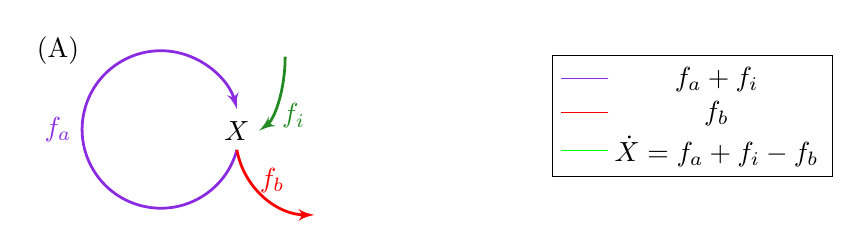
\begin{tikzpicture}[>=latex',node distance = 2cm]
            \node (X) {$X$};
            \draw [->,line width=1pt,BlueViolet] (X.south) arc (345:15:1cm) node [pos=0.5,left] (fa) {$f_a$};
            \draw [->,line width=1pt,red] (X.south) arc (190:270:1cm) node [pos=0.3,right] {$f_b$};
            \draw [<-,line width=1pt,ForestGreen] (X.east) arc (-70:0:0.5cm and 1cm) node [pos=0.3,right] (fi) {$f_i$};
            \node [above of=fa,yshift=-1cm] (A) {(A)};
            \begin{customlegend}[legend entries={$f_a+f_i$,$f_b$,$\dot{X}=f_a+f_i-f_b$},legend style={right=3cm of fi,anchor=west,name=legend1}]
              \addlegendimage{BlueViolet,fill=black!50!red,sharp plot}
              \addlegendimage{red,fill=black!50!red,sharp plot}
              \addlegendimage{green,fill=black!50!red,sharp plot}
            \end{customlegend}
         \end{tikzpicture}}%
       \end{minipage}

       \begin{minipage}[c]{\linewidth}%
        {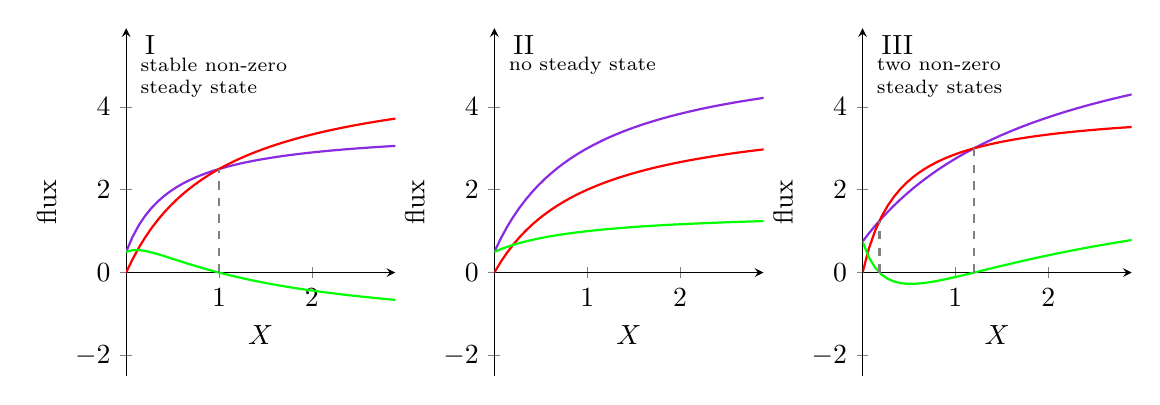
\begin{tikzpicture}
            \begin{axis}[name=plot1,axis x line=middle,axis y line=left,xlabel near ticks,ylabel near ticks,xmin=0,ymin=-2.5,xmax=2.9,ymax=5.9,xlabel={$X$},ylabel={flux},samples=60,width=5cm,height=6cm]
            \addplot[domain=0:4,BlueViolet,thick] {3*x/(0.5+x)+\influx};
            \addplot[domain=0:4,red,thick] {5*x/(1+x)};
            \addplot[domain=0:4,green,thick] {3*x/(0.5+x)-5*x/(1+x)+\influx};
            \addplot[dashed,gray,thick] coordinates {(1,0) (1,2.5)};
            \node[right] (one) at (axis cs:0.1,5.5) {I};
            \node[right,align=left] (onetext) at (axis cs:0.05,4.7) {\scriptsize stable non-zero\\[-0.4em]\scriptsize steady state};
          \end{axis}

          \begin{axis}[name=plot2,axis x line=middle,axis y line=left,xlabel near ticks,ylabel near ticks,xmin=0,ymin=-2.5,xmax=2.9,ymax=5.9,xlabel={$X$},ylabel={flux},samples=60,at=(plot1.right of south east),anchor=left of south west,width=5cm,height=6cm]
            \addplot[domain=0:4,BlueViolet,thick] {5*x/(1+x)+\influx};
            \addplot[domain=0:4,red,thick] {4*x/(1+x)};
            \addplot[domain=0:4,green,thick] {5*x/(1+x)-4*x/(1+x)+\influx};
            \node[right] (two) at (axis cs:0.1,5.5) {II};
            \node[right,align=left] (twotext) at (axis cs:0.05,5) {\scriptsize no steady state};
          \end{axis}

          \begin{axis}[name=plot3,axis x line=middle,axis y line=left,xlabel near ticks,ylabel near ticks,xmin=0,ymin=-2.5,xmax=2.9,ymax=5.9,xlabel={$X$},ylabel={flux},samples=60,at=(plot2.right of south east),anchor=left of south west,width=5cm,height=6cm]
            \addplot[domain=0:4,BlueViolet,thick] {6*x/(2+x)+1.5*\influx};
            \addplot[domain=0:4,red,thick] {4*x/(0.4+x)};
            \addplot[domain=0:4,green,thick] {6*x/(2+x)-4*x/(0.4+x)+1.5*\influx};
            \addplot[dashed,gray,thick] coordinates {(1.2,0) (1.2,3)};
            \addplot[dashed,gray,thick] coordinates {(0.182,0) (0.182,1.25)};
            \node[right] (three) at (axis cs:0.1,5.5) {III};
            \node[right,align=left] (threetext) at (axis cs:0.05,4.7) {\scriptsize two non-zero\\[-0.4em]\scriptsize steady states};
          \end{axis}
        \end{tikzpicture}}
       \end{minipage}
      \caption{\label{fig:inputcycle}
        (A) A simple autocatalytic cycle with a fixed input flux, $f_i$.
        A steady state occurs when $f_a+f_i=f_b$.
        If $V_{\max,b}>V_{\max,a}+f_i$ then there is always a single stable steady state (I).
        If $V_{\max,b}<V_{\max,a}+f_i$ then there can either be no steady states (II), or two steady states where the smaller one is stable (III).
      }
    \end{figure}
    \subsection{Using different kinetics equations}
    We used simple, irreversible Michaelis-Menten kinetics equation as this equation is the most widely used equation to model enzyme kinetics.
    However, our results can be extended to different kinetic equations.
    For different equations one must calculate the positive concentrations at which the two fluxes (the autocatalytic reaction and the biomass generating reaction) intercept.
    If such interception point(s) exist, the stability condition remains as before, i.e. that an interception point is stable if and only if the biomass generating reaction has higher elasticity at the given concentration.
    \subsection{Stability analysis for longer simple cycles (optional)}
    It is useful to extend the simple criteria we derived for more complex autocatalytic cycles.
    The most straightforward extension is for cycles with more than one intermediate metabolite.
    We start by writing the relevant equations for a two-metabolite autocatalytic cycle depicted in figure \ref{fig:longcycle}.
    In this system there are two intermediate metabolites, $X_1$ and $X_2$, two reactions that form the cycle, $f_{a_1}$ and $f_{a_2}$, and two biomass generating reactions, $f_{b_1}$ and $f_{b_2}$.
    We arbitrarily assume that the autocatalytic reaction is $f_{a_1}$ and that the autocaltalysis is in a $1:2$ ratio.
    Given that a steady state of the system exists for some value $X_1^*,X_2^*$ we can evaluate the expression for stability.
    In multi-variable system stability dictates that the real part of the eigenvalues of the Jacobian matrix must all be negative for a steady state to be stable.
    We define $\alpha_i=\frac{\partial f_{a_i}}{\partial X_i}$ and $\beta_i=\frac{\partial f_{b_i}}{\partial X_i}$ for $i=1,2$ and get that:
    \begin{equation*}
        J=
        \begin{pmatrix}
            -(\alpha_1+\beta_1) & \alpha_2 \\
            2\alpha_1 & -(\alpha_2+\beta_2)
        \end{pmatrix}
    \end{equation*}
    Solving for the characteristic polynomial gives:
    \begin{align}
        0 & =(\lambda+\alpha_1+\beta_1)(\lambda+\alpha_2+\beta_2)-2\alpha_1\alpha_2 \\
        & = \lambda^2+(\alpha_1+\beta_1+\alpha_2+\beta_2)\lambda+(\alpha_1+\beta_1)(\alpha_2+\beta_2)-2\alpha_1\alpha_2
    \end{align}
    which has two negative roots when:
    \begin{equation}
        (\alpha_1+\beta_1)(\alpha_2+\beta_2)-2\alpha_1\alpha_2>0
    \end{equation}
    The condition is strongly met if $\beta_1\geq \alpha_1$ and $\beta_2\geq\alpha_2$.
    
    The two-metabolites cycle case can be easily extended for a larger number of intermediate metabolites and reactions giving a general characteristic polynomial of:
    \begin{equation}
        0=\prod_{i=1}^n(\lambda+\alpha_i+\beta_i)-2\prod_{i=1}^n\alpha_i
    \end{equation}

    \section{Testing the predictions of the analysis on the identified autocatalytic cycles}
    To evaluate the validity of our analysis of autocatalytic cycles we searched for growth conditions under which the autocatalytic cycles we identified in central carbon metabolism carry substantial flux.
    We used recent in-vivo flux measurements from \cite{Gerosa2015-oq}.
    According to the data, two autocatalytic cycles carry substantial flux under at least one of the growth conditions:
    the glyoxilate cycle carries significant flux at growth in galactose and acetate;
    the PTS using cycle carries significant flux at growth in glucose.
    As for the other classes of autocatalytic cycles we note that the pentose-phosphate cycle variants do not carry flux in any of the tested conditions, which is not surprising given the non-standard metabolites they assimilate.
    The reverse FBA with ED pathway cycle did not carry flux in any of the measured conditions either.
    Although glycerol could have been a good carbon source to use this pathway, the metabolic network allows for a more energy efficient growth by following the common lower glycolysis reactions from GAP to pyruvate, avoiding the need to use the less energy efficient ED pathway.
    The CBB cycle, which is not a part of the metabolic network of wild type \emph{E.coli},  has been recently introduced synthetically into \emph{E.coli} and was shown to carry flux in it, given further metabolic engineering of central carbon metabolism \cite{Antonovski2016}.

    In the two cycles for which we were able to identify growth conditions under which substantial flux flows through the autocatalytic cycles we again used the data from \cite{Gerosa2015-oq} to identify the major branching points in the cycle.
    The branching points are highlighted in figure \ref{fig:branch}.

    Having identified the relevant growth conditions and branching points, we tested, for each combination of growth condition, active cycle, and major branching point, whether the stability criteria holds.
    To that end we checked which of the two reactions - the branching reaction or the cycle reaction, carried a larger flux compared with the reaction capacity, given the $k_\text{cat}$ values of the reactions and the amount of enzymes expressed at that condition.

    We used data from \cite{Schmidt2015} for the expression level, and data from \cite{BRENDA/Davidi} for the $k_\text{cat}$ values.
    In all 6 cases observed there was an agreement between the calculated capacity usage relationships and the predictions based on the stability criteria of lower capacity usage for the branching reaction compared with the cycle reaction ($P=1/2^6=0.015$).
    Our results are summarized in table \ref{tab1}
    growth condition    | branch-point substrate    | branching enzyme | cycle enzyme   | branching enzyme vmax* | cycle enzyme vmax* | branching enzyme km | cycle enzyme km   | branching enzyme vmax/km | cycle enzyme vmax/km |
    Galactoes           | isocitrate                | icd              | aceA/glcB      |                        |                    | 0.029 (brd 1.1.1.42)| non-available     |
    Galactoes           | oxaloacetate              | pck              | glt            |                        |                    | 670 (brd 4.1.1.49)  |
    Acetate             | isocitrate                | icd              | aceA/glcB      |                        |                    | 0.029               | non-available     |
    Acetate             | oxaloacetate              | ppck             | glt            |                        |                    |
    Glucose             | glucose 6 phospate        | zwf              | pgi            |                        |                    |
    

    name km kcat ec

    Glyoxilate cycle, bottom:
    icd, 0.029 (conditions?), 106 kcat, 11kmax, 1.1.1.42 (km from brnd, kcat from davidi)
    aceA, 0.015/0.09, not available, 4.1.3.1

    Glyoxilate cycle, top:
    pck, 0.67 , 0.67?, 4.1.1.49
    glt, 0.02, 81 kcat, 58 kmax, 2.3.3.16

    PTS cycle, glucose, top:
    zwf, 0.174, 174, 1.1.1.49, reversible, from bar-even/flamholz
    pgi, 0.28, 120, 5.3.1.9, reversible, from bar-even/flamholz

    PTS cycle, fructose, top (ask elad how to consolidate more than 100\% and the two fructose PTS's:
    fbp
    fba/B, 0.17, 10, 4.1.2.13, reversible, from bar-even/flamholz

    PTS cycle: ppc+pyk vs. PTS

    For the CBB cycle we restate the observation made in \cite{Antonovski2016} according to which changes in the kinetic properties of the main branching reaction out of the CBB pathway, PRS, were essential to produce a hemi-autotrophic strain relying on flux through the CBB pathway.

    To conclude, while thorough knowledge of the kinetic properties, concentrations and fluxes under various growth conditions is still sparse, we were able to verify that existing data supports preditions made by our model, given the requirement for stable steady state operation of autocatalytic cycles.
\begin{figure}[h!]
\centering
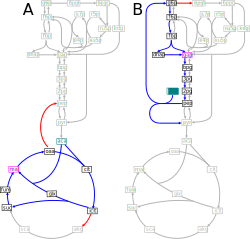
\includegraphics[scale=0.86]{central-carbon-met-fig2.pdf}
    \caption {
        Major branching points of the autocatalytic cycles under growth conditions where they carry flux.
        The branching reactions are marked in red.
(A) The glyoxylate cycle carries substantial flux under growth in galactose or acetate.
(B) The PTS using cycle carries substantial flux under grwoth in glucose.}
    \label{fig:branch}
\end{figure}


\section{Discussion}
A common concept in synthetic biology is that the successful implementation of novel pathways requires the expression of functional enzymes in the correct amounts in the target organism.
Here we show that in the specific context of the newly introduced enzymes being involved in autocatalytic cycles, such a successful expression may not suffice.
Specifically, changes to some of the kinetic parameters of enzymes may be required in order for the novel pathway to function.

Another aspect of our findings is that while generally, high affinity and catalytic rate are desirable traits for enzymes, in the specific context of autocatalytic cycles, constraints may exist on the relations between these kinetic parameters across different enzymes rendering improvements in only some of them deleterious for the functioning of the cycle.

A recent demonstration of these principles in vivo is the implementation of a functional CBB cycle in \emph{e.coli} by introducing the two genes missing for its functioning \cite{Antonovski2016}.
The successful introduction of the genes did not suffice to make the cycle function, and further directed evolution was needed in order to achieve non-zero flux.
A key change in the evolutionary process was the decrease of the affinity of phosphoribosylpyrophosphate synthetase (PRS), one of the enzymes responsible for the flux out of the CBB cycle, corresponding to the biomass reaction in our simple model.

Our observation regarding the stabilizing effect of input fluxes into an autocatalytic cycle may provide some means to mitigate the stability issue allowing for a pathway to gradually evolve towards sustainable flux.

Qualitatively, whereas in usual metabolic context a higher flux through a reaction will not decrease the flux into any of its reactants (it may increase this flux if one of the reactions feeding into the reactant is reversible), in setups involving autocatalytic cycles, such negative feedback exists as an inherent structural feature of the system.

While autocatalytic cycles are usually considered a small part of metabolism, with less than a handful of examples, we note that by the definition presented here, such cycles are abundant even in central carbon metabolism.
The examples of autocatalytic cycles we provide, as well as our verified predictions on the economical usage of enzymes catalyzing reactions branching out of such cycles suggest that the constraints we find on the kinetic parameters of enzymes involved in autocatalytic cycles may confine and shape the kinetic parameters of a broad set of enzymes central to metabolism.

\section{Acknowledgments}
We would like to thank Arren Bar-Even, Katja Tummler, Daniel Segre, Matthias Heinemann, David Fell, Patrick Shih, Wolfram Liebermeister  and \dots for fruitful discussions and valuable insights contributing to this work.
\bibliography{library}{}
\bibliographystyle{ieeetr}
\end{document}
